\section{Luồng hoạt động}

\begin{figure}[H]
	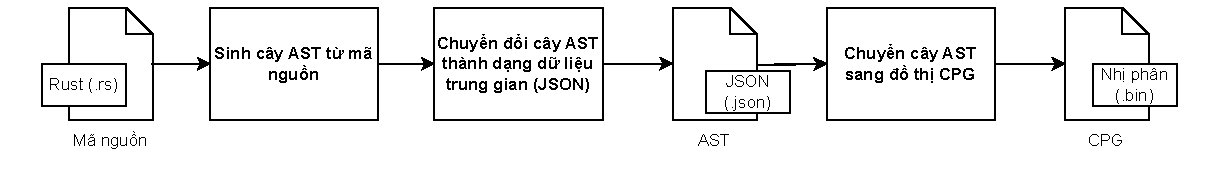
\includegraphics[width=1\columnwidth]{figures/c3/c3_flow_2.drawio.pdf}
	\centering
	\caption{Quy trình phân tích mã nguồn Rust.}
	\label{img:c3_flow_2}
\end{figure}

% \begin{figure}[H]
% 	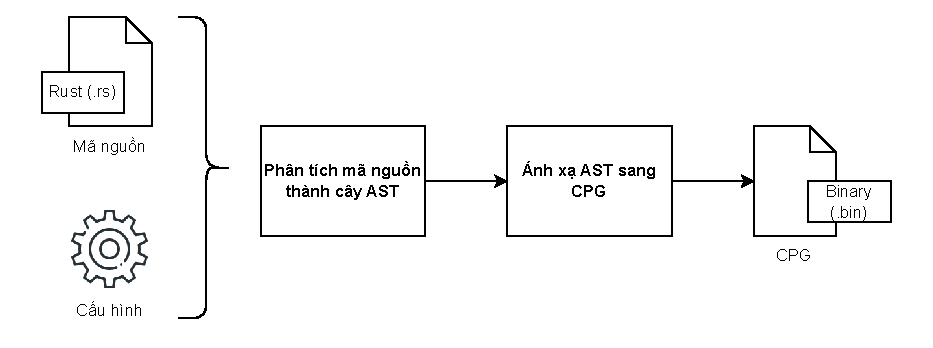
\includegraphics[width=1\columnwidth]{figures/c3/c3_flow.drawio.pdf}
% 	\centering
% 	\caption{Quy trình phân tích mã nguồn Rust.}
% 	\label{img:c3_flow}
% \end{figure}

% \begin{figure}[H]
% 	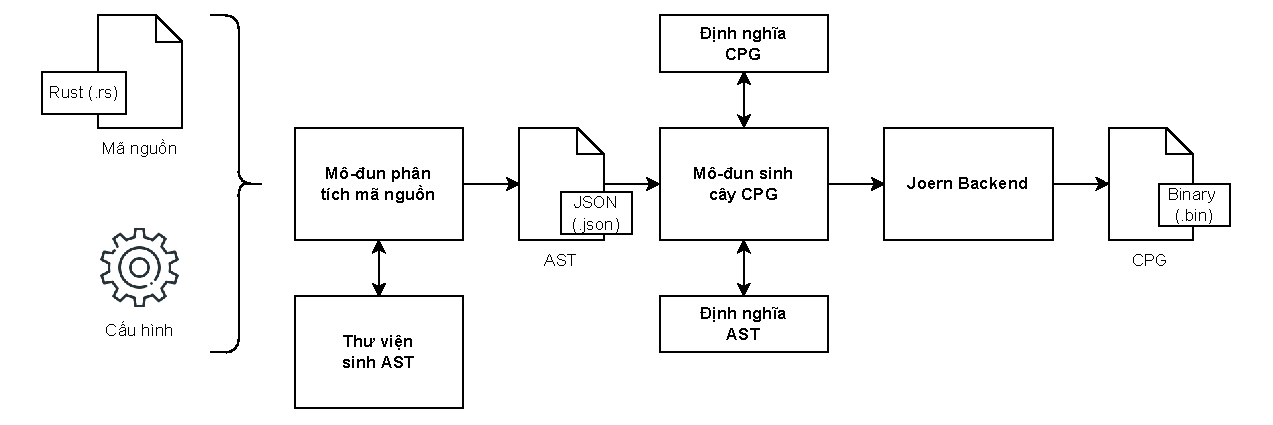
\includegraphics[width=1\columnwidth]{figures/c4/c4_install_flow.drawio.pdf}
% 	\centering
% 	\caption{Kiến trúc công cụ.}
% 	\label{img:c4_install_flow}
% \end{figure}

% \begin{figure}[H]
% 	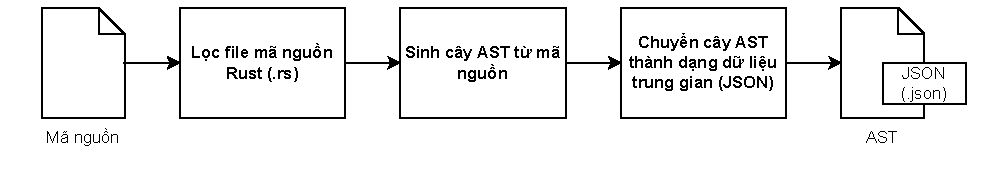
\includegraphics[width=1\columnwidth]{figures/c3/c3_flow_ast.drawio.pdf}
% 	\centering
% 	\caption{Quy trình xây dựng cây AST.}
% 	\label{img:c3_flow_ast}
% \end{figure}z

Mục tiêu của công cụ là phân tích mã nguồn Rust và xây dựng đồ thị CPG biểu diễn mã nguồn đó.
Đầu vào của công cụ là các tệp mã nguồn Rust, đầu ra là đồ thị CPG lưu dưới dạng nhị phân.
Đồ thị CPG được phục vụ cho việc thực hiện các câu lệnh truy vấn trên đồ thị hoặc quét đồ thị để tìm lỗ hổng trong mã nguồn.
Với yêu cầu đầu vào, đầu ra như trên, luồng hoạt động của công cụ bao gồm các bước được thể hiện trong hình \ref{img:c3_flow_2}.
Chi tiết các bước được tiến hành như sau:

\begin{enumerate}
	\item Từ thư mục của dự án, lọc lấy các tệp mã nguồn Rust (các tệp có đuôi \texttt{.rs}).
	\item Với mỗi tệp mã nguồn, sử dụng thư viện \textit{syn} \cite{synRust} để sinh cây AST từ nội dung mã nguồn của tệp đó.
	\textit{syn} là một thư viện phân tích mã nguồn thành cây AST được sử dụng rộng rãi với nhiều mục đích, trong đó bao gồm việc cài đặt tính năng Procedural Macro \cite{rustlangProceduralMacros} của Rust.
	Tính tới thời điểm hiện tại Rust không có đặc tả ngôn ngữ chính thức, do đó cộng đồng sử dụng Rust Reference \cite{rustReference} coi như phiên bản sát nhất so với một đặc tả ngôn ngữ.
	Thư viện syn xây dựng định nghĩa các nút của cây AST tuân theo Rust Reference.
	\item Chuyển đổi cây AST từ ngôn ngữ Rust sang định dạng JSON.
	Joern có thể được sử dụng cho nhiều ngôn ngữ và Joern Frontend không phụ thuộc vào bộ phân tích ngôn ngữ của một ngôn ngữ nhất định, do vậy cần có định dạng dữ liệu trung gian để chuyển đổi cây AST của bộ phân tích ngôn ngữ sang ngôn ngữ Scala của Joern Frontend.
	Có các kiểu dữ liệu trung gian phổ biến như JSON, XML, YAML, trong đó JSON được lựa chọn bởi tính đơn giản, dễ chuyển đổi.
	\item Cây AST dưới định dạng JSON được đọc ngược lại bằng mã nguồn Scala của Joern Frontend.
	Từ đây ta sẽ thực hiện chuyển đổi cây AST sang đồ thị CPG, từng loại nút trong cây AST sẽ có ánh xạ tương ứng với một loại nút trong đồ thị CPG.
	Các thông tin trong cây AST sẽ được khai thác để xây dựng nút CPG phù hợp, thông tin giữa các nút AST được sử dụng để xây dựng các cạnh, thuộc tính cho cạnh và nút trong đồ thị CPG.
	Quá trình xây dựng đồ thị CPG sẽ bao gồm vai trò của Joern Frontend và Joern Backend, quá trình này sẽ được mô tả chi tiết ở phần \ref{chapter:arch}.
	\item Cuối cùng, đồ thị CPG được lưu dưới dạng tệp nhị phân và đây là đầu ra kì vọng của công cụ.
\end{enumerate}